% English poster companion to poster.tex.
\documentclass[17pt,a1paper,portrait,margin=0mm,innermargin=12mm,
  blockverticalspace=8mm,colspace=10mm,titletotopverticalspace=2mm]{tikzposter}
\usepackage[utf8]{inputenc}
\usepackage[T1]{fontenc}
\usepackage[english]{babel}
\usepackage{amsmath,amssymb,graphicx,tikz}
\usetikzlibrary{arrows.meta,positioning,shapes.geometric,fit}
\definecolor{mainblue}{RGB}{15,55,110}
\definecolor{lightblue}{RGB}{210,225,245}
\definecolor{accentred}{RGB}{180,30,30}
\definecolor{darkgray}{RGB}{60,60,60}
\definecolor{blockbg}{RGB}{245,248,255}
\usetheme{Default}
\colorlet{backgroundcolor}{white}
\colorlet{blocktitlebgcolor}{mainblue}
\colorlet{blocktitlefgcolor}{white}
\colorlet{blockbodybgcolor}{blockbg}
\colorlet{blockbodyfgcolor}{black}
\colorlet{titlefgcolor}{mainblue}
\colorlet{titlebgcolor}{white}
\newcommand{\score}{s_\theta}
\newcommand{\dd}{\,\mathrm{d}}
\title{}\author{}\institute{}
\makeatletter
\renewcommand{\TP@maketitle}{\centering{\color{titlefgcolor}
  {\bfseries\Huge\sc Score-based diffusion models\par}\vspace{0.15em}
  {\Large The mathematics behind modern generative models\par}\vspace{0.25em}
  {\huge Gonzalo Josué Spina\par}\vspace{0.15em}
  {\large University of Buenos Aires \textbullet\ Faculty of Exact and Natural Sciences \textbullet\ Stochastic Calculus, 2026}}}
\makeatother
\begin{document}\maketitle\begin{columns}
\column{0.30}
\block{1. The problem}{
\textbf{Goal:} generate new samples from an unknown data distribution $p_0(x)$.\\[4pt]
We progressively corrupt observed samples with noise until reaching a known prior $\pi$, then learn how to reverse the process.
}
\block{2. Diffusions as generative models}{
The forward process is an Itô SDE:
\[\dd X_t=u(t,X_t)\dd t+\sigma(t,X_t)\dd B_t,\qquad X_0\sim p_0.\]
For a suitable drift and diffusion coefficient, the process can be ergodic: for large $T$, $X_T$ forgets the initial distribution and $p_T$ approaches a tractable stationary prior. Anderson's time-reversal result then adds the score to the reverse drift.
}
\block{3. Forward process: Ornstein--Uhlenbeck}{
\[\dd X_t=-X_t\dd t+\sigma\dd B_t.\]
The stable drift contracts the process while Brownian noise spreads mass. For large $T$, $p_T\approx\mathcal N(0,\sigma^2/2)$.
\begin{center}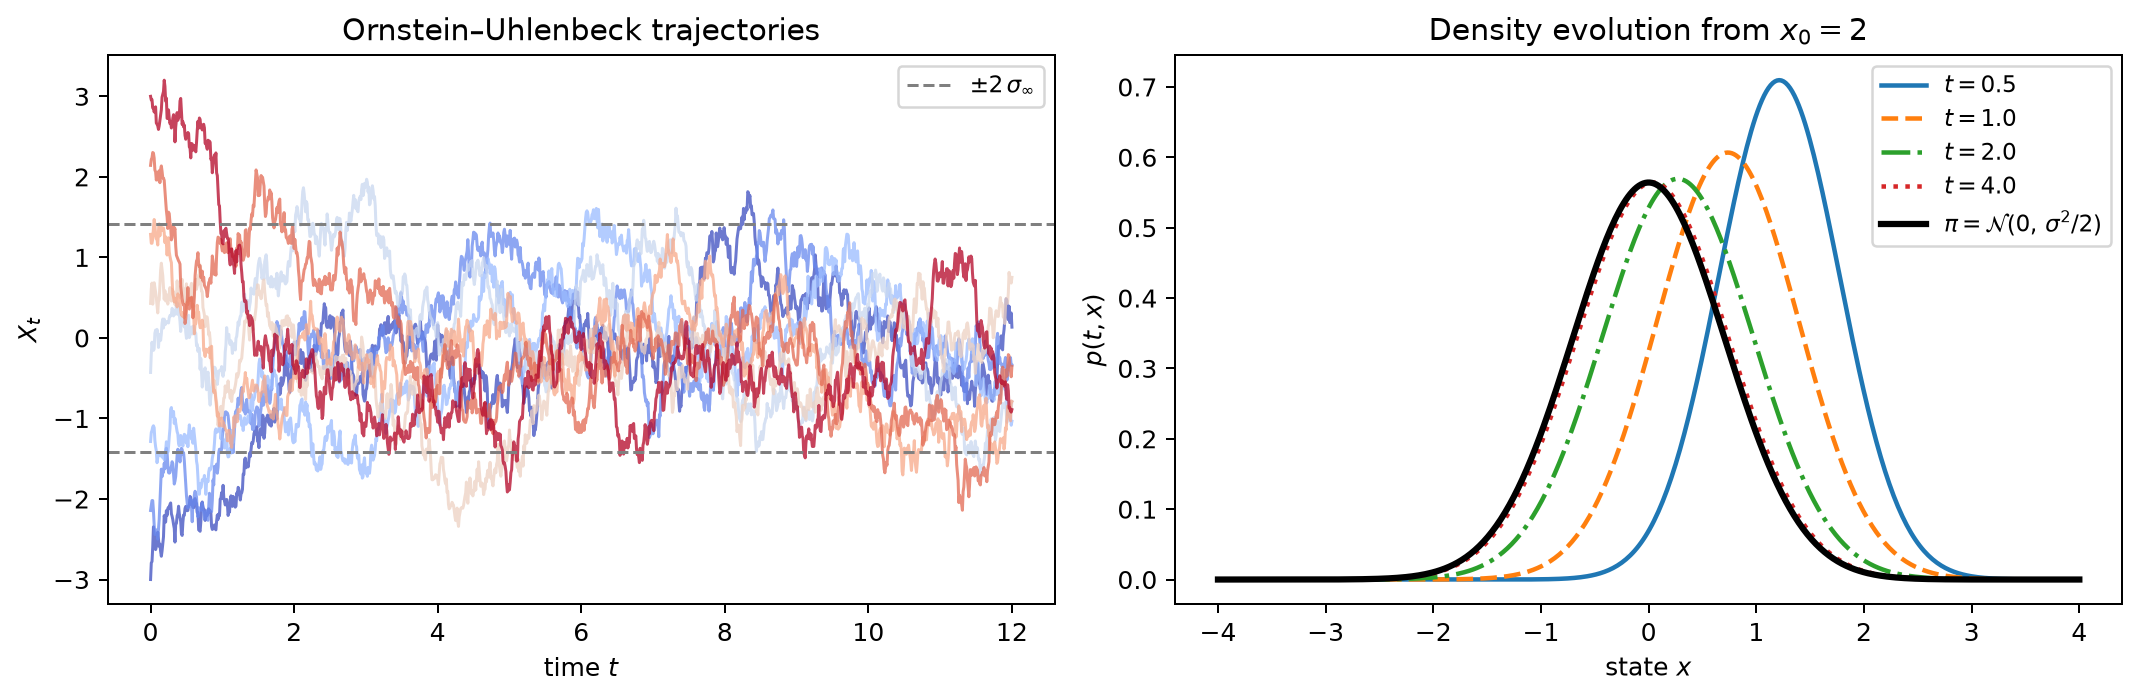
\includegraphics[width=.97\linewidth]{ou_trajectories_en.png}\end{center}}
\column{0.43}
\block{4. Anderson (1982): reverse time}{
\[\dd\hat X_\tau=\left[\hat X_\tau+\sigma^2\,\color{accentred}{\nabla_x\log p_{T-\tau}}\right]\dd\tau+\sigma\dd\bar B_\tau.\]
\begin{center}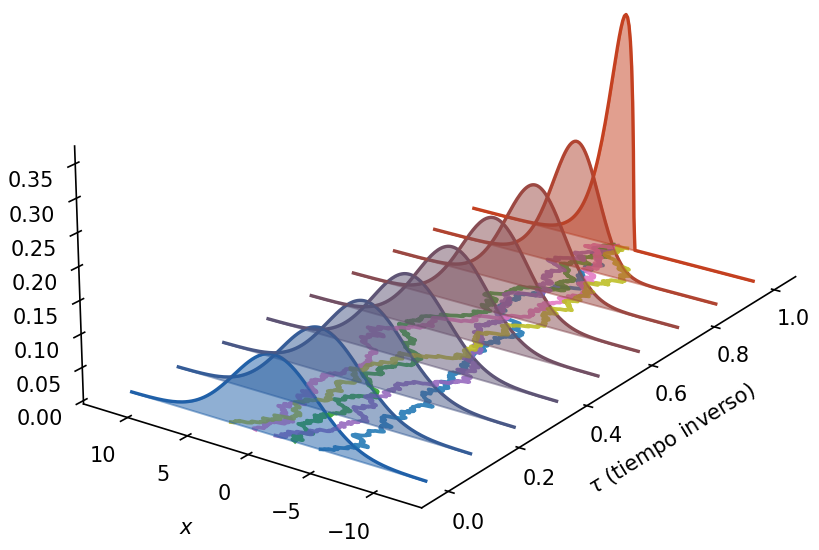
\includegraphics[width=.97\linewidth]{fig3_reverse_sde.png}\end{center}}
\block{5. The score}{
The unknown field $\color{accentred}{\nabla_x\log p_t(x)}$ is the score. It points toward higher-probability regions and supplies the correction that guides reverse diffusion.
\begin{center}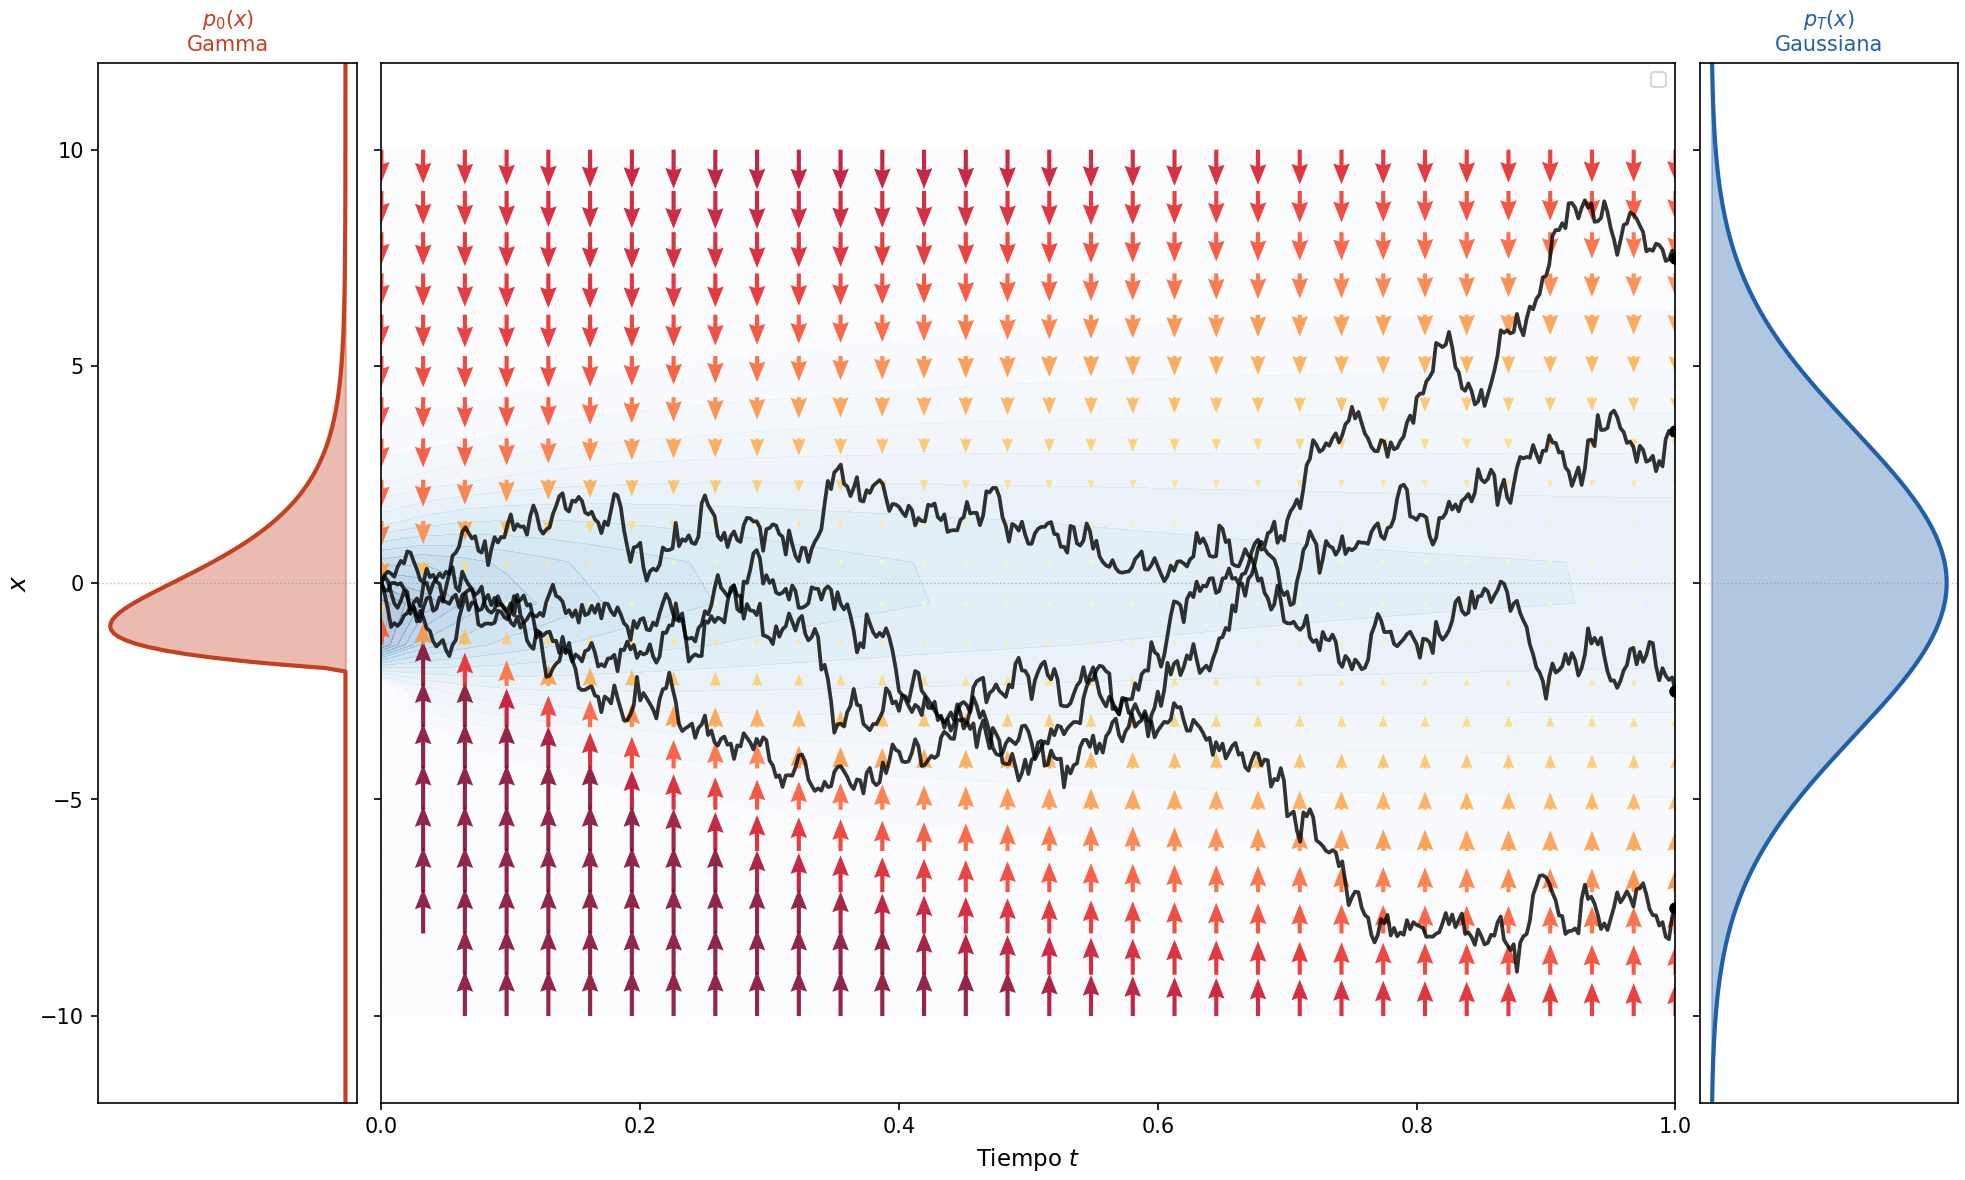
\includegraphics[width=.97\linewidth]{fig2_score.png}\end{center}
\textbf{Learning target:} $\score(x,t)\approx\nabla_x\log p_t(x)$.}
\block{6. Learning the score}{
The conditional score of a Gaussian corruption kernel is known:
\[\nabla_{\tilde x}\log q_\sigma(\tilde x\mid x)=-\frac{\tilde x-x}{\sigma^2}.\]
Denoising score matching trains a neural network against this target across noise levels. The network learns a vector field, not a normalized density.}
\column{0.27}
\block{7. What does the network learn?}{
\begin{center}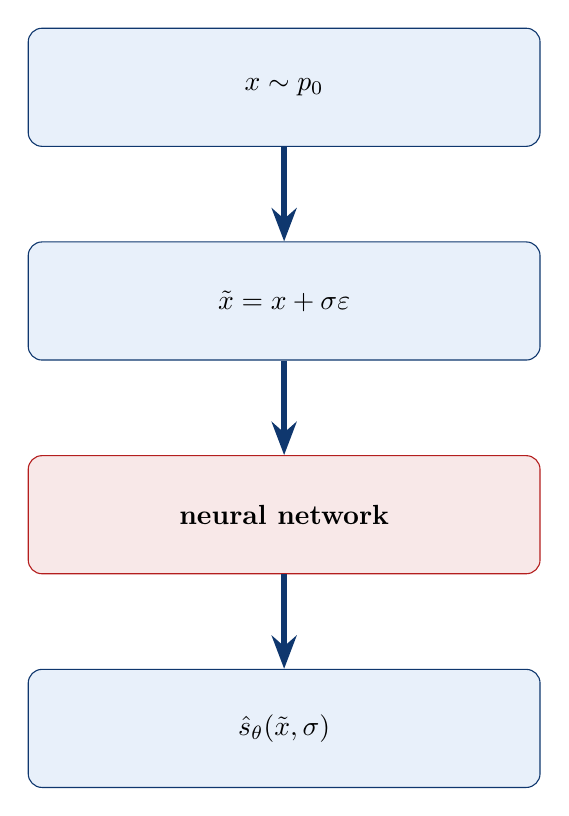
\begin{tikzpicture}[node distance=12mm,box/.style={draw=mainblue,fill=lightblue!50,rounded corners=5pt,minimum width=65mm,minimum height=15mm,font=\normalsize,align=center},redbox/.style={draw=accentred,fill=accentred!10,rounded corners=5pt,minimum width=65mm,minimum height=15mm,font=\normalsize\bfseries,align=center},arr/.style={-{Stealth},mainblue,line width=2pt}]
\node[box](x){$x\sim p_0$};\node[box,below=of x](xn){$\tilde x=x+\sigma\varepsilon$};\node[redbox,below=of xn](net){neural network};\node[box,below=of net](out){$\hat s_\theta(\tilde x,\sigma)$};\draw[arr](x)--(xn);\draw[arr](xn)--(net);\draw[arr](net)--(out);\end{tikzpicture}\end{center}}
\subcolumn{0.49}
\block{8. Probability-flow ODE}{
The reverse dynamics also admit a deterministic ODE with the same marginals:
\[\dd\hat X_\tau=\left[\hat X_\tau+\tfrac{\sigma^2}{2}\color{accentred}{\nabla_x\log p_{T-\tau}}\right]\dd\tau.\]
\begin{center}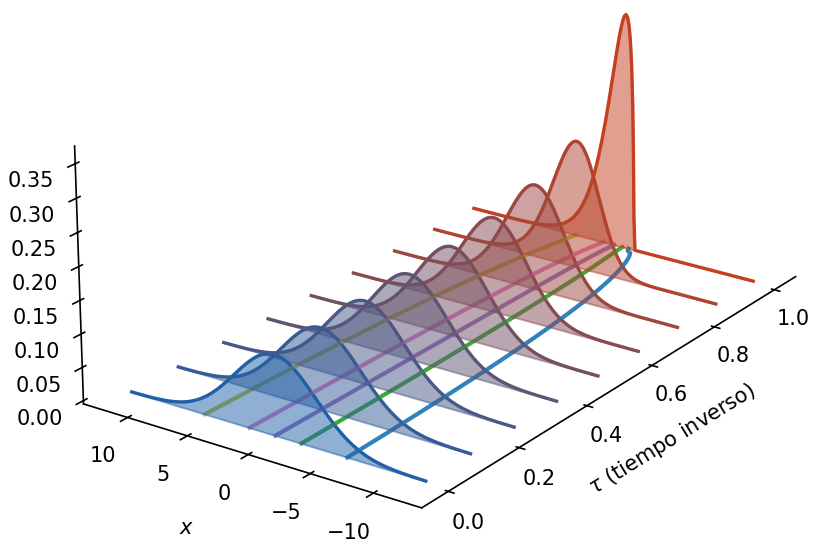
\includegraphics[width=.97\linewidth]{fig4_pflow.png}\end{center}}
\block{9. The pipeline works}{
Sample from the Gaussian prior, integrate the reverse SDE or probability-flow ODE, and obtain an approximation to $p_0$.
\begin{center}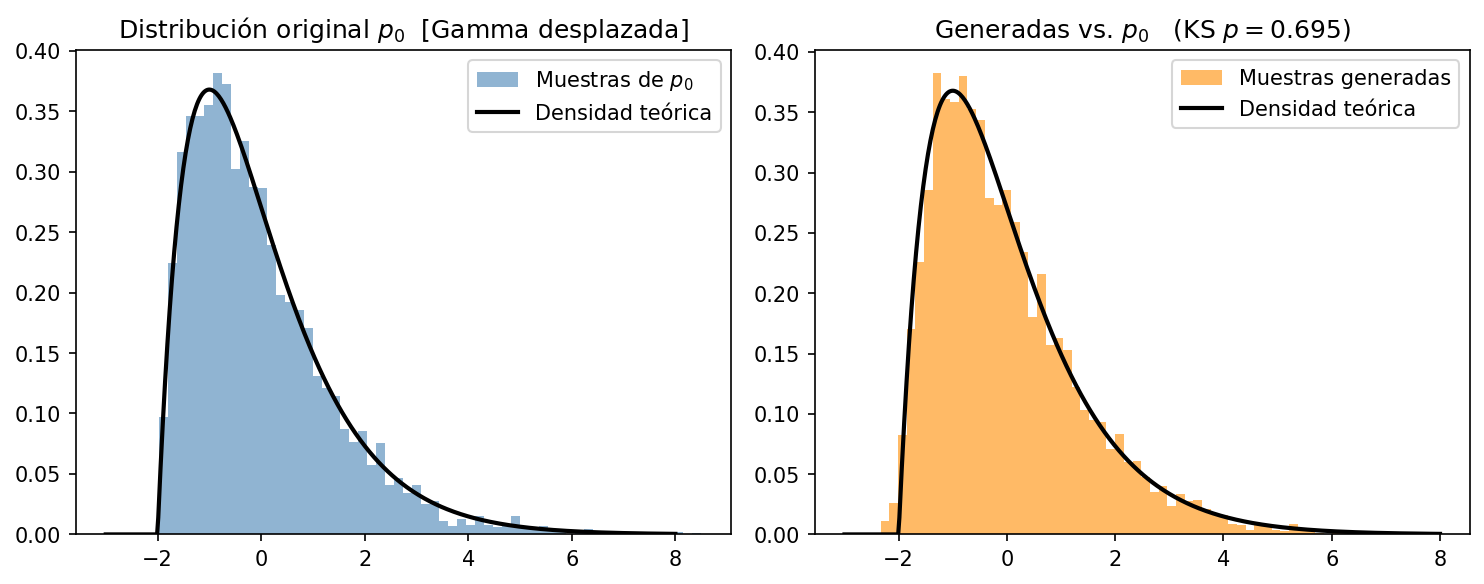
\includegraphics[width=.90\linewidth]{score_matching_demo.png}\end{center}
\begin{center}{\color{mainblue}KS test: $p=0.695$; the null is not rejected.\\[4pt]\textbf{Geometry + probability + deep learning.}}\end{center}}
\end{columns}\end{document}
